\section{Discretely-Optimised VQE}

\subsubsection{Excitation Operators in ZXC}

Let's look again at the parametrised single-body unitary operator,

\begin{equation*}
\begin{gathered}
    U^q_p (\theta) =
    \text{exp} \left( i
    \frac{\theta}{2} (Y_p X_q - X_p Y_q) \prod_{k=p+1}^{q-1} Z_k \right) \\
    %
    U^q_p (\theta) =
    \left( \text{exp} \left[
    i \frac{\theta}{2} Y_p X_q \prod_{k=p+1}^{q-1} Z_k \right] \right)
    %
    \left( \text{exp} \left[ -
    i \frac{\theta}{2} X_p Y_q \prod_{k=p+1}^{q-1} Z_k \right] \right)
\end{gathered}
\end{equation*}

The first exponential term can be implemented by the following phase gadget.
\begin{equation*}
    \text{exp} \left( i
    \frac{\theta}{2} Y_p X_q \prod_{k=p+1}^{q-1} Z_k \right)
\end{equation*}

% \begin{figure}
% \centering
%     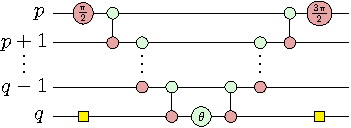
\includegraphics[width=8cm]{figures/zxc/yx_cnot}
% \end{figure}

% Rotation of qubit $p$ into $Y$ basis and rotation of qubit $q$ into $X$ basis, followed rotations back into $Z$ basis at the end of the circuit.

% Left CNOT ladder construction calculates the parity of the qubit state, and applies a rotation in the $Z$ basis if the parity is odd.

% Right CNOT ladder construction to uncompute.

Whilst the second exponential term can be implemented by the phase gadget.
\begin{equation*}
    \text{exp} \left( - i
    \frac{\theta}{2} X_p Y_q \prod_{k=p+1}^{q-1} Z_k \right)
\end{equation*}

% \begin{figure}
% \centering
%     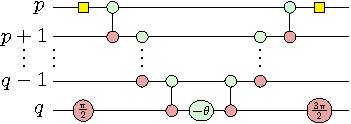
\includegraphics[width=8cm]{figures/zxc/xy_cnot}
% \end{figure}

%%% ----- %%%

Together, they constitute the single-body unitary excitation operator $U^q_p (\theta)$

% \begin{figure}
% \centering
%     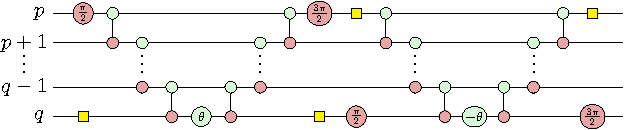
\includegraphics[width=14cm]{figures/zxc/full_cnot}
% \end{figure}

By defining the ordering of spin-orbitals such that adjacent spin-orbitals share the same spatial orbital, adjacent single-body operators commute.

\begin{equation*}
    \left[ \hat\kappa_p^q, \hat\kappa_{p+1}^{q+1} \right] = 0
\end{equation*}\smallskip

The same is therefore true for the resulting qubit operators,

\begin{equation*}
\begin{gathered}
    \left[ F_p^q, F_{p+1}^{q+1} \right] = 0 \\
    p, q \in \text{even} \qquad p+1, q+1 \in \text{odd}
\end{gathered}
\end{equation*}

This allows us to define the parametrised unitary qubit operators in terms of spin-adapted excitation operators.

\begin{equation*}
    U^q_p (\theta) = \text{exp}
    \left[ \theta \left( F_p^q + F_{p+1}^{q+1} \right) \right]
\end{equation*}

In other words, since $F_p^q$ and $F_{p+1}^{q+1}$ commute, we can think of them as a single operator with a single parameter.

